\section{External evaluation on measured drone flights}
\label{sec:external}

\subsection{Data, held-out trajectories, and physical prior}

We extend the controlled study to the NanoDrone benchmark, which records
Crazyflie 2.1 Brushless flights using motion capture and onboard sensors
\cite{busetto2026_nanodrone}. The released records include the authors'
offline synchronization, 100\,Hz resampling, motor--acceleration alignment,
and zero-phase low-pass filtering. We retain these records and predict their
recorded state estimates. Position, velocity, rotation-vector orientation,
and body angular velocity form a 12-coordinate state; four motor angular
speeds are the inputs.

Complete flights define the split. Runs 1--3 of Square, Random, and Chirp
provide nine training records (41,700 samples); run 4 of each supplies three
validation records (13,899 samples). Three Melon flights (19,497 samples)
test a trajectory family absent from training. This validation holdout is an
addition to the authors' training/test partition. Windows remain within
flights, and normalization uses training samples only.

The nominal model combines gravity with thrust along the body vertical axis:
\begin{equation}
 a_t=c_T R(r_t)e_3\sum_{j=1}^{4}\omega_{j,t}^{2}-g e_3,
 \qquad
 v_{t+1}=v_t+\Delta t\,a_t,\quad
 p_{t+1}=p_t+\Delta t\,v_t+\tfrac12\Delta t^2a_t.
 \label{eq:flight-prior}
\end{equation}
Here $r_t$ is the rotation vector, $\omega_{j,t}$ is motor speed,
$g=9.81\,\mathrm{m\,s^{-2}}$, and $\Delta t=0.01$\,s. A nonnegative
least-squares fit on training transitions gives
$c_T=8.31887655\times10^{-7}$ in
$(\mathrm{m\,s^{-2}})/(\mathrm{rad\,s^{-1}})^2$.
Orientation advances by quaternion composition under constant body angular
velocity. The prior omits angular acceleration, drag, and motor lag, adding
structural mismatch to the parameter mismatch studied in the simulations.

\subsection{Matched comparisons and evaluation protocol}

The flight implementation uses a width-64 recurrent encoder and residual
transition. Three learned models share \ExternalLearnedParameters{} parameters:
CFR-WM with gain 0.5, an unfiltered physics-residual model, and a data-only
recurrent transition. The latter replaces the nominal physics step with a
learned increment; the unfiltered model starts from the final imputed
measurement. All three use the same encoder, bounded correction, and
diagonal-Gaussian likelihood. The context GRU receives 40 features; a
width-64 GRU cell advances the hidden state from 12 predicted coordinates and
four inputs. An $80\!\to\!64\!\to\!64\!\to\!24$ SiLU head outputs
12 corrections and 12 log variances. Corrections use $0.25\tanh(\cdot)$ in
normalized coordinates, and log variances are clipped to $[-8,4]$.
A nominal-only forecast supplies a fourth
reference. These matched implementations follow the physics, hybrid, and
recurrent families represented in the NanoDrone benchmark.

Each window contains eight context states. Last-value imputation and elapsed
missingness times are computed within each flight before window extraction,
so an imputed entry can retain an observation preceding the eight-state
context. Training uses an equal mixture of recorded contexts and contexts
with Gaussian noise of 0.05 training standard deviations per coordinate and
10\% independent missingness. Controls and targets are unchanged. All learned
models train on 25-step rollouts with stride 10, AdamW, batch size 256, at most
40 epochs, and eight-epoch early stopping. Each method selects between
learning rates 0.001 and 0.003 by validation NLL using development seed 17,
then trains with five final seeds (131, 149, 167, 181, 199).

Evaluation uses four paired context conditions: as recorded, Gaussian noise
only (0.1 training standard deviations), missingness only (30\%), and their
combination. The same perturbation realization is shared across methods and
training seeds. Known recorded motor inputs drive free forecasts through
25 and 50 steps (0.25 and 0.5\,s), with test stride 50. For flight $f$, model
$m$, and horizon $H$, the external score is
\begin{equation}
 E_{m,f,H}=\sqrt{\frac{1}{12H N_f}
 \sum_{i=1}^{N_f}\sum_{h=1}^{H}\sum_{d=1}^{12}
 \left(\frac{\widehat{x}_{m,i,h,d}-x_{i,h,d}}{s_d}\right)^2},
 \label{eq:external-score}
\end{equation}
where $s_d$ is the training standard deviation. This score takes one root
after pooling normalized squared errors; the controlled study instead
averages feature-wise normalized RMSE. External summaries first give the
three flights equal weight, then report the mean and sample SD across five
training seeds. Position and velocity scores use root-mean-square Euclidean
error in physical units. Paired relative improvements are averaged across
seeds after the same flight weighting.

The flight protocol was recorded before external test evaluation and executed
after the synthetic confirmation. Its descriptive comparisons extend the
empirical setting while retaining the original H1 and H2 decisions.

\subsection{Flight forecasting results}

Table~\ref{tab:external-results} reports all eight condition--horizon
comparisons. Each learned model has lower mean full-state NRMSE than the
nominal forecast. The unfiltered residual model has lower mean full-state
NRMSE than CFR-WM in all eight comparisons. With recorded contexts at 50 steps,
their scores are \ExternalUnfilteredRecordedLongNRMSEMean{} and
\ExternalCFRRecordedLongNRMSEMean{}, respectively. Combined noise and
missingness narrows this difference to
\ExternalUnfilteredCombinedLongNRMSEMean{} versus
\ExternalCFRCombinedLongNRMSEMean{}.
CFR-WM improves over the data-only recurrent model at 25 steps under added
noise and combined corruption, but its mean error is higher at 50 steps
in all four conditions.

The physical-unit scores distinguish position and velocity behavior
(Table~\ref{tab:external-physical}; Figure~\ref{fig:external-flight}).
CFR-WM has the lowest 50-step position error among the three learned models
in all four conditions. Under combined corruption, its position error is
\ExternalCFRCombinedLongPositionMean{}\,m, compared with
\ExternalUnfilteredCombinedLongPositionMean{}\,m for the unfiltered model.
The nominal prior has lower position error than the learned models on
recorded and missing-only contexts, despite its higher full-state error.
Velocity errors show a different ordering: CFR-WM is worse than the
unfiltered model on recorded and missing-only contexts, and nearly tied
under noise and combined corruption. Thus, the position benefit coexists
with a full-state accuracy cost on these held-out flights.

\begin{table*}[t]
\centering
\caption{External flight NRMSE (Equation~\ref{eq:external-score}). Entries
are means $\pm$ SD across five training seeds after equal weighting of three
held-out flights. The nominal forecast is deterministic. All four context
conditions and both horizons are retained.}
\label{tab:external-results}
\resizebox{\textwidth}{!}{\input{../table_external_results}}
\end{table*}

\begin{table*}[t]
\centering
\caption{External 50-step position and velocity error in physical units,
using the same flight and seed weighting as Table~\ref{tab:external-results}.}
\label{tab:external-physical}
\resizebox{\textwidth}{!}{\input{../table_external_physical}}
\end{table*}

\begin{figure*}[t]
\centering
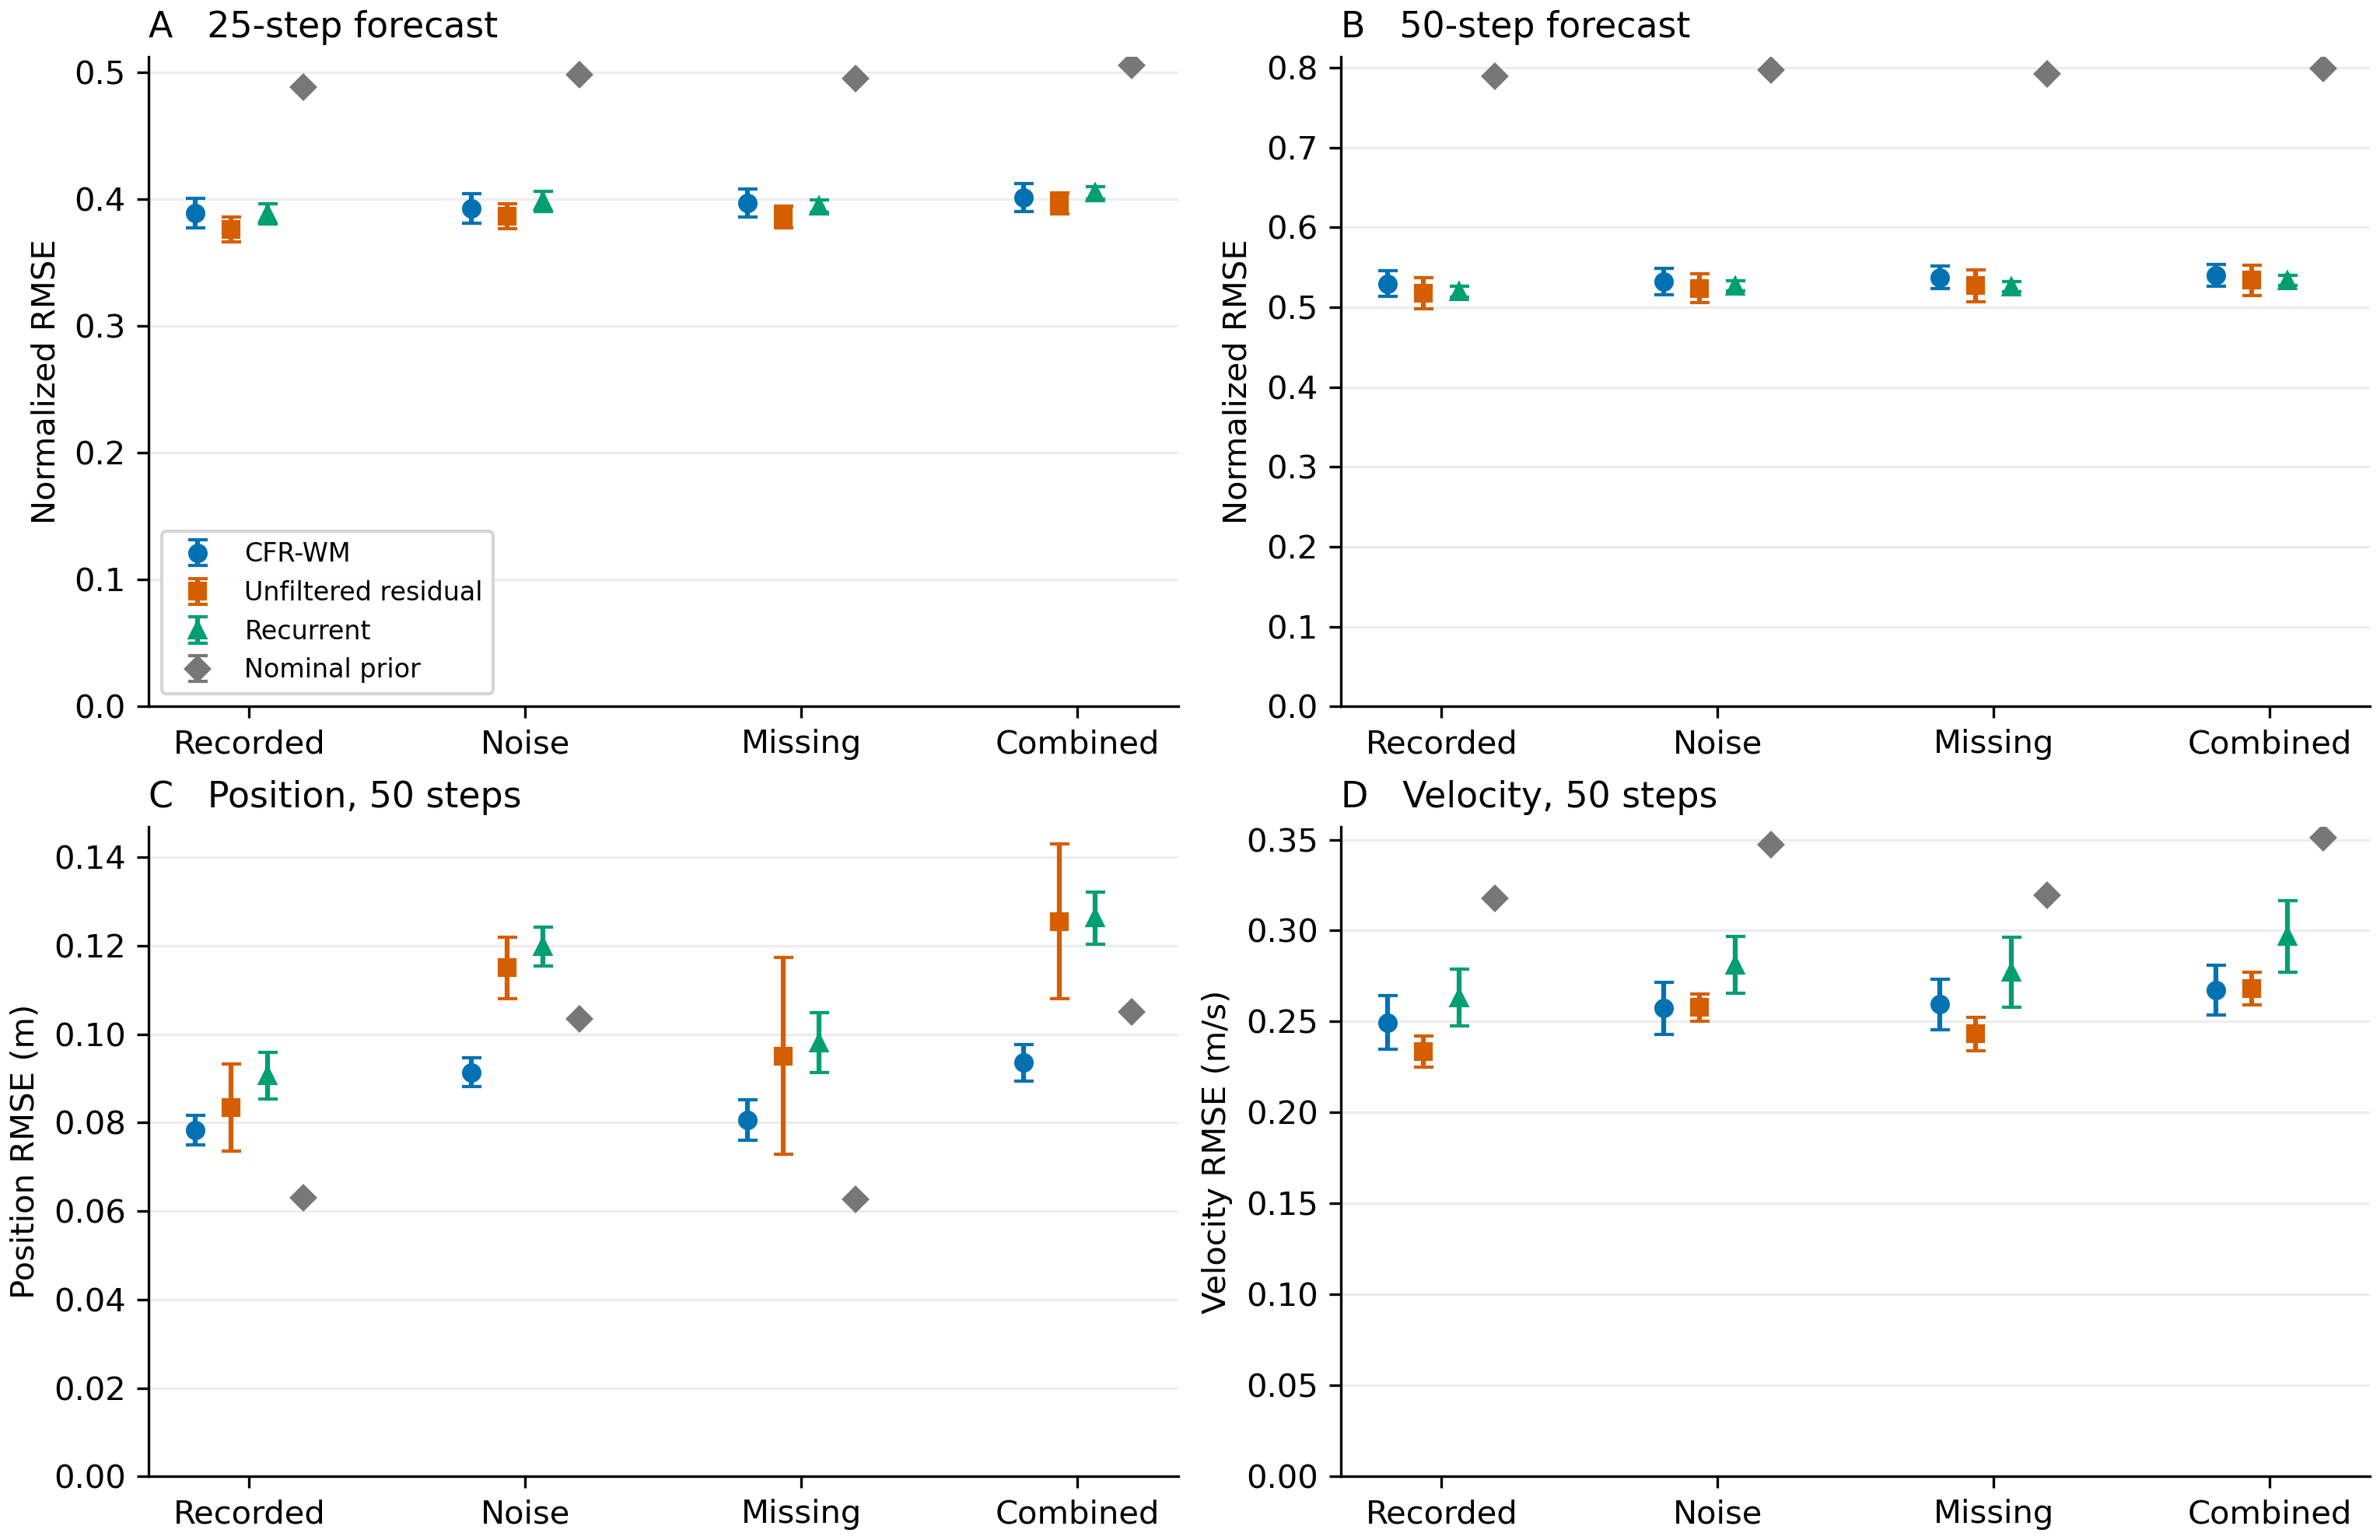
\includegraphics[width=\textwidth]{figures/external_flight.png}
\caption{Prediction on the held-out Melon flights: both normalized-error
horizons and 50-step position and velocity errors. Error bars describe
training-seed variation on the same three test flights.}
\label{fig:external-flight}
\end{figure*}
